\documentclass[1p]{elsarticle_modified}
%\bibliographystyle{elsarticle-num}

%\usepackage[colorlinks]{hyperref}
%\usepackage{abbrmath_seonhwa} %\Abb, \Ascr, \Acal ,\Abf, \Afrak
\usepackage{amsfonts}
\usepackage{amssymb}
\usepackage{amsmath}
\usepackage{amsthm}
\usepackage{scalefnt}
\usepackage{amsbsy}
\usepackage{kotex}
\usepackage{caption}
\usepackage{subfig}
\usepackage{color}
\usepackage{graphicx}
\usepackage{xcolor} %% white, black, red, green, blue, cyan, magenta, yellow
\usepackage{float}
\usepackage{setspace}
\usepackage{hyperref}

\usepackage{tikz}
\usetikzlibrary{arrows}

\usepackage{multirow}
\usepackage{array} % fixed length table
\usepackage{hhline}

%%%%%%%%%%%%%%%%%%%%%
\makeatletter
\renewcommand*\env@matrix[1][\arraystretch]{%
	\edef\arraystretch{#1}%
	\hskip -\arraycolsep
	\let\@ifnextchar\new@ifnextchar
	\array{*\c@MaxMatrixCols c}}
\makeatother %https://tex.stackexchange.com/questions/14071/how-can-i-increase-the-line-spacing-in-a-matrix
%%%%%%%%%%%%%%%

\usepackage[normalem]{ulem}

\newcommand{\msout}[1]{\ifmmode\text{\sout{\ensuremath{#1}}}\else\sout{#1}\fi}
%SOURCE: \msout is \stkout macro in https://tex.stackexchange.com/questions/20609/strikeout-in-math-mode

\newcommand{\cancel}[1]{
	\ifmmode
	{\color{red}\msout{#1}}
	\else
	{\color{red}\sout{#1}}
	\fi
}

\newcommand{\add}[1]{
	{\color{blue}\uwave{#1}}
}

\newcommand{\replace}[2]{
	\ifmmode
	{\color{red}\msout{#1}}{\color{blue}\uwave{#2}}
	\else
	{\color{red}\sout{#1}}{\color{blue}\uwave{#2}}
	\fi
}

\newcommand{\Sol}{\mathcal{S}} %segment
\newcommand{\D}{D} %diagram
\newcommand{\A}{\mathcal{A}} %arc


%%%%%%%%%%%%%%%%%%%%%%%%%%%%%5 test

\def\sl{\operatorname{\textup{SL}}(2,\Cbb)}
\def\psl{\operatorname{\textup{PSL}}(2,\Cbb)}
\def\quan{\mkern 1mu \triangleright \mkern 1mu}

\theoremstyle{definition}
\newtheorem{thm}{Theorem}[section]
\newtheorem{prop}[thm]{Proposition}
\newtheorem{lem}[thm]{Lemma}
\newtheorem{ques}[thm]{Question}
\newtheorem{cor}[thm]{Corollary}
\newtheorem{defn}[thm]{Definition}
\newtheorem{exam}[thm]{Example}
\newtheorem{rmk}[thm]{Remark}
\newtheorem{alg}[thm]{Algorithm}

\newcommand{\I}{\sqrt{-1}}
\begin{document}

%\begin{frontmatter}
%
%\title{Boundary parabolic representations of knots up to 8 crossings}
%
%%% Group authors per affiliation:
%\author{Yunhi Cho} 
%\address{Department of Mathematics, University of Seoul, Seoul, Korea}
%\ead{yhcho@uos.ac.kr}
%
%
%\author{Seonhwa Kim} %\fnref{s_kim}}
%\address{Center for Geometry and Physics, Institute for Basic Science, Pohang, 37673, Korea}
%\ead{ryeona17@ibs.re.kr}
%
%\author{Hyuk Kim}
%\address{Department of Mathematical Sciences, Seoul National University, Seoul 08826, Korea}
%\ead{hyukkim@snu.ac.kr}
%
%\author{Seokbeom Yoon}
%\address{Department of Mathematical Sciences, Seoul National University, Seoul, 08826,  Korea}
%\ead{sbyoon15@snu.ac.kr}
%
%\begin{abstract}
%We find all boundary parabolic representation of knots up to 8 crossings.
%
%\end{abstract}
%\begin{keyword}
%    \MSC[2010] 57M25 
%\end{keyword}
%
%\end{frontmatter}

%\linenumbers
%\tableofcontents
%
\newcommand\colored[1]{\textcolor{white}{\rule[-0.35ex]{0.8em}{1.4ex}}\kern-0.8em\color{red} #1}%
%\newcommand\colored[1]{\textcolor{white}{ #1}\kern-2.17ex	\textcolor{white}{ #1}\kern-1.81ex	\textcolor{white}{ #1}\kern-2.15ex\color{red}#1	}

{\Large $\underline{12a_{0825}~(K12a_{0825})}$}

\setlength{\tabcolsep}{10pt}
\renewcommand{\arraystretch}{1.6}
\vspace{1cm}\begin{tabular}{m{100pt}>{\centering\arraybackslash}m{274pt}}
\multirow{5}{120pt}{
	\centering
	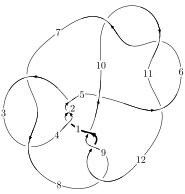
\includegraphics[width=112pt]{../../../GIT/diagram.site/Diagrams/png/1626_12a_0825.png}\\
\ \ \ A knot diagram\footnotemark}&
\allowdisplaybreaks
\textbf{Linearized knot diagam} \\
\cline{2-2}
 &
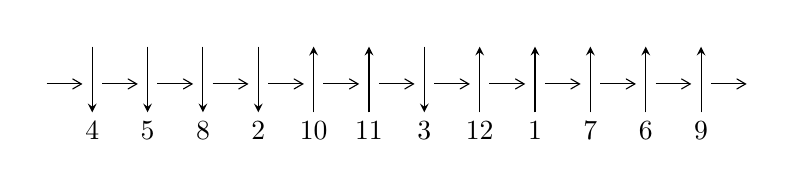
\begin{tikzpicture}[x=20pt, y=17pt]
	% nodes
	\node (C0) at (0, 0) {};
	\node (C1) at (1, 0) {};
	\node (C1U) at (1, +1) {};
	\node (C1D) at (1, -1) {4};

	\node (C2) at (2, 0) {};
	\node (C2U) at (2, +1) {};
	\node (C2D) at (2, -1) {5};

	\node (C3) at (3, 0) {};
	\node (C3U) at (3, +1) {};
	\node (C3D) at (3, -1) {8};

	\node (C4) at (4, 0) {};
	\node (C4U) at (4, +1) {};
	\node (C4D) at (4, -1) {2};

	\node (C5) at (5, 0) {};
	\node (C5U) at (5, +1) {};
	\node (C5D) at (5, -1) {10};

	\node (C6) at (6, 0) {};
	\node (C6U) at (6, +1) {};
	\node (C6D) at (6, -1) {11};

	\node (C7) at (7, 0) {};
	\node (C7U) at (7, +1) {};
	\node (C7D) at (7, -1) {3};

	\node (C8) at (8, 0) {};
	\node (C8U) at (8, +1) {};
	\node (C8D) at (8, -1) {12};

	\node (C9) at (9, 0) {};
	\node (C9U) at (9, +1) {};
	\node (C9D) at (9, -1) {1};

	\node (C10) at (10, 0) {};
	\node (C10U) at (10, +1) {};
	\node (C10D) at (10, -1) {7};

	\node (C11) at (11, 0) {};
	\node (C11U) at (11, +1) {};
	\node (C11D) at (11, -1) {6};

	\node (C12) at (12, 0) {};
	\node (C12U) at (12, +1) {};
	\node (C12D) at (12, -1) {9};
	\node (C13) at (13, 0) {};

	% arrows
	\draw[->,>={angle 60}]
	(C0) edge (C1) (C1) edge (C2) (C2) edge (C3) (C3) edge (C4) (C4) edge (C5) (C5) edge (C6) (C6) edge (C7) (C7) edge (C8) (C8) edge (C9) (C9) edge (C10) (C10) edge (C11) (C11) edge (C12) (C12) edge (C13) ;	\draw[->,>=stealth]
	(C1U) edge (C1D) (C2U) edge (C2D) (C3U) edge (C3D) (C4U) edge (C4D) (C5D) edge (C5U) (C6D) edge (C6U) (C7U) edge (C7D) (C8D) edge (C8U) (C9D) edge (C9U) (C10D) edge (C10U) (C11D) edge (C11U) (C12D) edge (C12U) ;
	\end{tikzpicture} \\
\hhline{~~} \\& 
\textbf{Solving Sequence} \\ \cline{2-2} 
 &
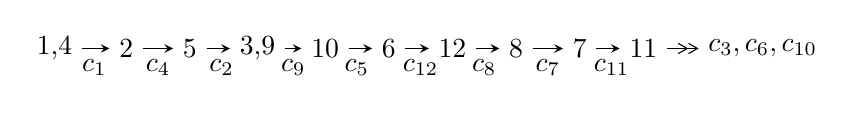
\begin{tikzpicture}[x=23pt, y=7pt]
	% node
	\node (A0) at (-1/8, 0) {1,4};
	\node (A1) at (1, 0) {2};
	\node (A2) at (2, 0) {5};
	\node (A3) at (49/16, 0) {3,9};
	\node (A4) at (33/8, 0) {10};
	\node (A5) at (41/8, 0) {6};
	\node (A6) at (49/8, 0) {12};
	\node (A7) at (57/8, 0) {8};
	\node (A8) at (65/8, 0) {7};
	\node (A9) at (73/8, 0) {11};
	\node (C1) at (1/2, -1) {$c_{1}$};
	\node (C2) at (3/2, -1) {$c_{4}$};
	\node (C3) at (5/2, -1) {$c_{2}$};
	\node (C4) at (29/8, -1) {$c_{9}$};
	\node (C5) at (37/8, -1) {$c_{5}$};
	\node (C6) at (45/8, -1) {$c_{12}$};
	\node (C7) at (53/8, -1) {$c_{8}$};
	\node (C8) at (61/8, -1) {$c_{7}$};
	\node (C9) at (69/8, -1) {$c_{11}$};
	\node (A10) at (11, 0) {$c_{3},c_{6},c_{10}$};

	% edge
	\draw[->,>=stealth]	
	(A0) edge (A1) (A1) edge (A2) (A2) edge (A3) (A3) edge (A4) (A4) edge (A5) (A5) edge (A6) (A6) edge (A7) (A7) edge (A8) (A8) edge (A9) ;
	\draw[->>,>={angle 60}]	
	(A9) edge (A10);
\end{tikzpicture} \\ 

\end{tabular} \\

\footnotetext{
The image of knot diagram is generated by the software ``\textbf{Draw programme}" developed by Andrew Bartholomew(\url{http://www.layer8.co.uk/maths/draw/index.htm\#Running-draw}), where we modified some parts for our purpose(\url{https://github.com/CATsTAILs/LinksPainter}).
}\phantom \\ \newline 
\centering \textbf{Ideals for irreducible components\footnotemark of $X_{\text{par}}$} 
 
\begin{align*}
I^u_{1}&=\langle 
3.79485\times10^{78} u^{79}+3.24042\times10^{79} u^{78}+\cdots+3.97586\times10^{76} b+2.32513\times10^{79},\\
\phantom{I^u_{1}}&\phantom{= \langle  }-1.11614\times10^{78} u^{79}-9.33264\times10^{78} u^{78}+\cdots+5.96379\times10^{76} a-5.21526\times10^{78},\\
\phantom{I^u_{1}}&\phantom{= \langle  }u^{80}+10 u^{79}+\cdots-61 u+9\rangle \\
I^u_{2}&=\langle 
-9 a^5+15 a^4+29 a^3-11 a^2+13 b-9 a-5,\;3 a^6+2 a^5-4 a^4-3 a^3+1,\;u-1\rangle \\
I^u_{3}&=\langle 
b+1,\;a^2-2 a u-4 a+9 u+15,\;u^2+u-1\rangle \\
I^u_{4}&=\langle 
b-1,\;a+u+2,\;u^2+u-1\rangle \\
\\
\end{align*}
\raggedright * 4 irreducible components of $\dim_{\mathbb{C}}=0$, with total 92 representations.\\
\footnotetext{All coefficients of polynomials are rational numbers. But the coefficients are sometimes approximated in decimal forms when there is not enough margin.}
\newpage
\renewcommand{\arraystretch}{1}
\centering \section*{I. $I^u_{1}= \langle 3.79\times10^{78} u^{79}+3.24\times10^{79} u^{78}+\cdots+3.98\times10^{76} b+2.33\times10^{79},\;-1.12\times10^{78} u^{79}-9.33\times10^{78} u^{78}+\cdots+5.96\times10^{76} a-5.22\times10^{78},\;u^{80}+10 u^{79}+\cdots-61 u+9 \rangle$}
\flushleft \textbf{(i) Arc colorings}\\
\begin{tabular}{m{7pt} m{180pt} m{7pt} m{180pt} }
\flushright $a_{1}=$&$\begin{pmatrix}1\\0\end{pmatrix}$ \\
\flushright $a_{4}=$&$\begin{pmatrix}0\\u\end{pmatrix}$ \\
\flushright $a_{2}=$&$\begin{pmatrix}1\\u^2\end{pmatrix}$ \\
\flushright $a_{5}=$&$\begin{pmatrix}- u\\- u^3+u\end{pmatrix}$ \\
\flushright $a_{3}=$&$\begin{pmatrix}- u^2+1\\- u^4+2 u^2\end{pmatrix}$ \\
\flushright $a_{9}=$&$\begin{pmatrix}18.7153 u^{79}+156.488 u^{78}+\cdots-649.568 u+87.4487\\-95.4474 u^{79}-815.023 u^{78}+\cdots+4365.64 u-584.812\end{pmatrix}$ \\
\flushright $a_{10}=$&$\begin{pmatrix}-76.7321 u^{79}-658.535 u^{78}+\cdots+3716.07 u-497.363\\-95.4474 u^{79}-815.023 u^{78}+\cdots+4365.64 u-584.812\end{pmatrix}$ \\
\flushright $a_{6}=$&$\begin{pmatrix}-78.4351 u^{79}-659.518 u^{78}+\cdots+3232.63 u-436.354\\-123.641 u^{79}-1086.82 u^{78}+\cdots+6687.09 u-885.806\end{pmatrix}$ \\
\flushright $a_{12}=$&$\begin{pmatrix}-91.7460 u^{79}-788.305 u^{78}+\cdots+4317.85 u-579.520\\87.9807 u^{79}+760.193 u^{78}+\cdots-4426.42 u+588.470\end{pmatrix}$ \\
\flushright $a_{8}=$&$\begin{pmatrix}-60.2340 u^{79}-518.813 u^{78}+\cdots+2900.90 u-389.646\\89.0583 u^{79}+756.154 u^{78}+\cdots-3964.33 u+532.844\end{pmatrix}$ \\
\flushright $a_{7}=$&$\begin{pmatrix}8.30253 u^{79}+82.9747 u^{78}+\cdots-735.274 u+93.4145\\32.0105 u^{79}+287.801 u^{78}+\cdots-1979.29 u+259.874\end{pmatrix}$ \\
\flushright $a_{11}=$&$\begin{pmatrix}-28.5574 u^{79}-246.679 u^{78}+\cdots+1502.25 u-199.834\\26.6383 u^{79}+236.438 u^{78}+\cdots-1600.04 u+209.994\end{pmatrix}$\\&\end{tabular}
\flushleft \textbf{(ii) Obstruction class $= -1$}\\~\\
\flushleft \textbf{(iii) Cusp Shapes $= -352.037 u^{79}-3003.98 u^{78}+\cdots+16150.8 u-2151.32$}\\~\\
\newpage\renewcommand{\arraystretch}{1}
\flushleft \textbf{(iv) u-Polynomials at the component}\newline \\
\begin{tabular}{m{50pt}|m{274pt}}
Crossings & \hspace{64pt}u-Polynomials at each crossing \\
\hline $$\begin{aligned}c_{1},c_{2},c_{4}\end{aligned}$$&$\begin{aligned}
&u^{80}-10 u^{79}+\cdots+61 u+9
\end{aligned}$\\
\hline $$\begin{aligned}c_{3},c_{7}\end{aligned}$$&$\begin{aligned}
&u^{80}-2 u^{79}+\cdots-2112 u+576
\end{aligned}$\\
\hline $$\begin{aligned}c_{5}\end{aligned}$$&$\begin{aligned}
&u^{80}+2 u^{79}+\cdots+17620 u+3460
\end{aligned}$\\
\hline $$\begin{aligned}c_{6},c_{10},c_{11}\end{aligned}$$&$\begin{aligned}
&u^{80}-2 u^{79}+\cdots-20 u+4
\end{aligned}$\\
\hline $$\begin{aligned}c_{8},c_{9},c_{12}\end{aligned}$$&$\begin{aligned}
&u^{80}-4 u^{79}+\cdots-61 u+19
\end{aligned}$\\
\hline
\end{tabular}\\~\\
\newpage\renewcommand{\arraystretch}{1}
\flushleft \textbf{(v) Riley Polynomials at the component}\newline \\
\begin{tabular}{m{50pt}|m{274pt}}
Crossings & \hspace{64pt}Riley Polynomials at each crossing \\
\hline $$\begin{aligned}c_{1},c_{2},c_{4}\end{aligned}$$&$\begin{aligned}
&y^{80}-78 y^{79}+\cdots+1139 y+81
\end{aligned}$\\
\hline $$\begin{aligned}c_{3},c_{7}\end{aligned}$$&$\begin{aligned}
&y^{80}-48 y^{79}+\cdots-8331264 y+331776
\end{aligned}$\\
\hline $$\begin{aligned}c_{5}\end{aligned}$$&$\begin{aligned}
&y^{80}+2 y^{79}+\cdots-459714960 y+11971600
\end{aligned}$\\
\hline $$\begin{aligned}c_{6},c_{10},c_{11}\end{aligned}$$&$\begin{aligned}
&y^{80}+74 y^{79}+\cdots-528 y+16
\end{aligned}$\\
\hline $$\begin{aligned}c_{8},c_{9},c_{12}\end{aligned}$$&$\begin{aligned}
&y^{80}-72 y^{79}+\cdots-12613 y+361
\end{aligned}$\\
\hline
\end{tabular}\\~\\
\newpage\flushleft \textbf{(vi) Complex Volumes and Cusp Shapes}
$$\begin{array}{c|c|c}  
\text{Solutions to }I^u_{1}& \I (\text{vol} + \sqrt{-1}CS) & \text{Cusp shape}\\
 \hline 
\begin{aligned}
u &= \phantom{-}0.746557 + 0.636954 I \\
a &= -0.682165 + 0.006700 I \\
b &= -0.145904 - 0.656703 I\end{aligned}
 & -6.94608 + 1.67535 I & \phantom{-0.000000 } 0 \\ \hline\begin{aligned}
u &= \phantom{-}0.746557 - 0.636954 I \\
a &= -0.682165 - 0.006700 I \\
b &= -0.145904 + 0.656703 I\end{aligned}
 & -6.94608 - 1.67535 I & \phantom{-0.000000 } 0 \\ \hline\begin{aligned}
u &= \phantom{-}0.378618 + 0.955753 I \\
a &= -2.00786 - 0.70595 I \\
b &= \phantom{-}1.39851 - 0.33871 I\end{aligned}
 & -0.68593 - 10.88960 I & \phantom{-0.000000 } 0 \\ \hline\begin{aligned}
u &= \phantom{-}0.378618 - 0.955753 I \\
a &= -2.00786 + 0.70595 I \\
b &= \phantom{-}1.39851 + 0.33871 I\end{aligned}
 & -0.68593 + 10.88960 I & \phantom{-0.000000 } 0 \\ \hline\begin{aligned}
u &= \phantom{-}1.020620 + 0.245504 I \\
a &= -0.88354 + 1.17817 I \\
b &= -0.505450 + 0.207652 I\end{aligned}
 & -5.18915 - 0.90638 I & \phantom{-0.000000 } 0 \\ \hline\begin{aligned}
u &= \phantom{-}1.020620 - 0.245504 I \\
a &= -0.88354 - 1.17817 I \\
b &= -0.505450 - 0.207652 I\end{aligned}
 & -5.18915 + 0.90638 I & \phantom{-0.000000 } 0 \\ \hline\begin{aligned}
u &= \phantom{-}0.295108 + 0.901425 I \\
a &= \phantom{-}2.22025 + 0.54370 I \\
b &= -1.40020 + 0.27744 I\end{aligned}
 & \phantom{-}4.80028 - 7.04030 I & \phantom{-0.000000 } 0 \\ \hline\begin{aligned}
u &= \phantom{-}0.295108 - 0.901425 I \\
a &= \phantom{-}2.22025 - 0.54370 I \\
b &= -1.40020 - 0.27744 I\end{aligned}
 & \phantom{-}4.80028 + 7.04030 I & \phantom{-0.000000 } 0 \\ \hline\begin{aligned}
u &= \phantom{-}0.394187 + 0.827178 I \\
a &= \phantom{-}0.425833 - 0.162336 I \\
b &= -0.220058 + 0.822245 I\end{aligned}
 & -5.82377 - 6.70367 I & \phantom{-0.000000 } 0 \\ \hline\begin{aligned}
u &= \phantom{-}0.394187 - 0.827178 I \\
a &= \phantom{-}0.425833 + 0.162336 I \\
b &= -0.220058 - 0.822245 I\end{aligned}
 & -5.82377 + 6.70367 I & \phantom{-0.000000 } 0\\
 \hline 
 \end{array}$$\newpage$$\begin{array}{c|c|c}  
\text{Solutions to }I^u_{1}& \I (\text{vol} + \sqrt{-1}CS) & \text{Cusp shape}\\
 \hline 
\begin{aligned}
u &= \phantom{-}0.889457\phantom{ +0.000000I} \\
a &= \phantom{-}0.660649\phantom{ +0.000000I} \\
b &= \phantom{-}0.159297\phantom{ +0.000000I}\end{aligned}
 & -1.24461\phantom{ +0.000000I} & \phantom{-0.000000 } 0 \\ \hline\begin{aligned}
u &= \phantom{-}0.965727 + 0.632385 I \\
a &= \phantom{-}1.269500 + 0.586728 I \\
b &= -1.324860 - 0.170371 I\end{aligned}
 & \phantom{-}2.78356 + 1.72362 I & \phantom{-0.000000 } 0 \\ \hline\begin{aligned}
u &= \phantom{-}0.965727 - 0.632385 I \\
a &= \phantom{-}1.269500 - 0.586728 I \\
b &= -1.324860 + 0.170371 I\end{aligned}
 & \phantom{-}2.78356 - 1.72362 I & \phantom{-0.000000 } 0 \\ \hline\begin{aligned}
u &= \phantom{-}0.894797 + 0.767292 I \\
a &= -1.196750 - 0.393590 I \\
b &= \phantom{-}1.349070 + 0.268437 I\end{aligned}
 & -2.22008 + 5.05652 I & \phantom{-0.000000 } 0 \\ \hline\begin{aligned}
u &= \phantom{-}0.894797 - 0.767292 I \\
a &= -1.196750 + 0.393590 I \\
b &= \phantom{-}1.349070 - 0.268437 I\end{aligned}
 & -2.22008 - 5.05652 I & \phantom{-0.000000 } 0 \\ \hline\begin{aligned}
u &= \phantom{-}0.209904 + 0.762735 I \\
a &= -2.71834 - 0.30206 I \\
b &= \phantom{-}1.363030 - 0.189174 I\end{aligned}
 & \phantom{-}3.27350 - 2.77001 I & \phantom{-0.000000 } 0 \\ \hline\begin{aligned}
u &= \phantom{-}0.209904 - 0.762735 I \\
a &= -2.71834 + 0.30206 I \\
b &= \phantom{-}1.363030 + 0.189174 I\end{aligned}
 & \phantom{-}3.27350 + 2.77001 I & \phantom{-0.000000 } 0 \\ \hline\begin{aligned}
u &= -1.21097\phantom{ +0.000000I} \\
a &= \phantom{-}1.37295\phantom{ +0.000000I} \\
b &= -1.62302\phantom{ +0.000000I}\end{aligned}
 & \phantom{-}5.30599\phantom{ +0.000000I} & \phantom{-0.000000 } 0 \\ \hline\begin{aligned}
u &= \phantom{-}0.349449 + 0.692603 I \\
a &= -0.468714 + 0.268886 I \\
b &= \phantom{-}0.262657 - 0.693020 I\end{aligned}
 & -0.48810 - 3.50449 I & \phantom{-0.000000 } 0 \\ \hline\begin{aligned}
u &= \phantom{-}0.349449 - 0.692603 I \\
a &= -0.468714 - 0.268886 I \\
b &= \phantom{-}0.262657 + 0.693020 I\end{aligned}
 & -0.48810 + 3.50449 I & \phantom{-0.000000 } 0\\
 \hline 
 \end{array}$$\newpage$$\begin{array}{c|c|c}  
\text{Solutions to }I^u_{1}& \I (\text{vol} + \sqrt{-1}CS) & \text{Cusp shape}\\
 \hline 
\begin{aligned}
u &= -1.221830 + 0.092628 I \\
a &= -1.38120 + 0.34319 I \\
b &= \phantom{-}1.59533 + 0.11935 I\end{aligned}
 & \phantom{-}1.44193 + 5.11024 I & \phantom{-0.000000 } 0 \\ \hline\begin{aligned}
u &= -1.221830 - 0.092628 I \\
a &= -1.38120 - 0.34319 I \\
b &= \phantom{-}1.59533 - 0.11935 I\end{aligned}
 & \phantom{-}1.44193 - 5.11024 I & \phantom{-0.000000 } 0 \\ \hline\begin{aligned}
u &= \phantom{-}1.216580 + 0.220859 I \\
a &= -0.81510 - 1.66598 I \\
b &= \phantom{-}1.233510 - 0.136855 I\end{aligned}
 & \phantom{-}0.291229 - 1.088620 I & \phantom{-0.000000 } 0 \\ \hline\begin{aligned}
u &= \phantom{-}1.216580 - 0.220859 I \\
a &= -0.81510 + 1.66598 I \\
b &= \phantom{-}1.233510 + 0.136855 I\end{aligned}
 & \phantom{-}0.291229 + 1.088620 I & \phantom{-0.000000 } 0 \\ \hline\begin{aligned}
u &= \phantom{-}1.254590 + 0.048642 I \\
a &= -0.47602 - 1.82196 I \\
b &= -1.064870 - 0.295239 I\end{aligned}
 & -5.76832 - 0.40080 I & \phantom{-0.000000 } 0 \\ \hline\begin{aligned}
u &= \phantom{-}1.254590 - 0.048642 I \\
a &= -0.47602 + 1.82196 I \\
b &= -1.064870 + 0.295239 I\end{aligned}
 & -5.76832 + 0.40080 I & \phantom{-0.000000 } 0 \\ \hline\begin{aligned}
u &= \phantom{-}1.170810 + 0.453578 I \\
a &= -1.07767 - 1.03396 I \\
b &= \phantom{-}1.338150 - 0.008543 I\end{aligned}
 & \phantom{-}0.41626 - 1.41355 I & \phantom{-0.000000 } 0 \\ \hline\begin{aligned}
u &= \phantom{-}1.170810 - 0.453578 I \\
a &= -1.07767 + 1.03396 I \\
b &= \phantom{-}1.338150 + 0.008543 I\end{aligned}
 & \phantom{-}0.41626 + 1.41355 I & \phantom{-0.000000 } 0 \\ \hline\begin{aligned}
u &= \phantom{-}0.337779 + 0.642636 I \\
a &= \phantom{-}1.45515 - 0.29598 I \\
b &= -0.988367 - 0.439985 I\end{aligned}
 & -3.47331 - 2.16270 I & \phantom{-0.000000 -}0. + 3.40294 I \\ \hline\begin{aligned}
u &= \phantom{-}0.337779 - 0.642636 I \\
a &= \phantom{-}1.45515 + 0.29598 I \\
b &= -0.988367 + 0.439985 I\end{aligned}
 & -3.47331 + 2.16270 I & \phantom{-0.000000 } 0. - 3.40294 I\\
 \hline 
 \end{array}$$\newpage$$\begin{array}{c|c|c}  
\text{Solutions to }I^u_{1}& \I (\text{vol} + \sqrt{-1}CS) & \text{Cusp shape}\\
 \hline 
\begin{aligned}
u &= \phantom{-}0.543823 + 0.447215 I \\
a &= \phantom{-}0.780717 - 0.230857 I \\
b &= -0.061345 + 0.440180 I\end{aligned}
 & -1.39076 - 0.43253 I & -3.80282 + 0. I\phantom{ +0.000000I} \\ \hline\begin{aligned}
u &= \phantom{-}0.543823 - 0.447215 I \\
a &= \phantom{-}0.780717 + 0.230857 I \\
b &= -0.061345 - 0.440180 I\end{aligned}
 & -1.39076 + 0.43253 I & -3.80282 + 0. I\phantom{ +0.000000I} \\ \hline\begin{aligned}
u &= -0.121092 + 0.686429 I \\
a &= -2.34739 + 0.92267 I \\
b &= \phantom{-}1.43204 - 0.01520 I\end{aligned}
 & \phantom{-}4.30728 - 2.43252 I & \phantom{-}5.74380 + 3.14176 I \\ \hline\begin{aligned}
u &= -0.121092 - 0.686429 I \\
a &= -2.34739 - 0.92267 I \\
b &= \phantom{-}1.43204 + 0.01520 I\end{aligned}
 & \phantom{-}4.30728 + 2.43252 I & \phantom{-}5.74380 - 3.14176 I \\ \hline\begin{aligned}
u &= \phantom{-}1.302040 + 0.087314 I \\
a &= \phantom{-}0.048944 - 0.999851 I \\
b &= \phantom{-}0.124215 - 0.610162 I\end{aligned}
 & -2.91730 - 1.56339 I & \phantom{-0.000000 } 0 \\ \hline\begin{aligned}
u &= \phantom{-}1.302040 - 0.087314 I \\
a &= \phantom{-}0.048944 + 0.999851 I \\
b &= \phantom{-}0.124215 + 0.610162 I\end{aligned}
 & -2.91730 + 1.56339 I & \phantom{-0.000000 } 0 \\ \hline\begin{aligned}
u &= -0.475431 + 0.460281 I \\
a &= -1.20403 + 1.49499 I \\
b &= \phantom{-}1.44724 + 0.20682 I\end{aligned}
 & \phantom{-}2.82742 + 5.64096 I & \phantom{-}5.82262 - 5.01289 I \\ \hline\begin{aligned}
u &= -0.475431 - 0.460281 I \\
a &= -1.20403 - 1.49499 I \\
b &= \phantom{-}1.44724 - 0.20682 I\end{aligned}
 & \phantom{-}2.82742 - 5.64096 I & \phantom{-}5.82262 + 5.01289 I \\ \hline\begin{aligned}
u &= -0.318513 + 0.576883 I \\
a &= \phantom{-}1.76623 - 1.41274 I \\
b &= -1.44334 - 0.10431 I\end{aligned}
 & \phantom{-}7.27651 + 1.62512 I & \phantom{-}9.82751 - 1.87978 I \\ \hline\begin{aligned}
u &= -0.318513 - 0.576883 I \\
a &= \phantom{-}1.76623 + 1.41274 I \\
b &= -1.44334 + 0.10431 I\end{aligned}
 & \phantom{-}7.27651 - 1.62512 I & \phantom{-}9.82751 + 1.87978 I\\
 \hline 
 \end{array}$$\newpage$$\begin{array}{c|c|c}  
\text{Solutions to }I^u_{1}& \I (\text{vol} + \sqrt{-1}CS) & \text{Cusp shape}\\
 \hline 
\begin{aligned}
u &= \phantom{-}0.373692 + 0.515975 I \\
a &= \phantom{-}4.02553 + 1.61667 I \\
b &= -1.198300 + 0.170105 I\end{aligned}
 & -3.93512 - 1.27756 I & \phantom{-}0.88119 + 5.42303 I \\ \hline\begin{aligned}
u &= \phantom{-}0.373692 - 0.515975 I \\
a &= \phantom{-}4.02553 - 1.61667 I \\
b &= -1.198300 - 0.170105 I\end{aligned}
 & -3.93512 + 1.27756 I & \phantom{-}0.88119 - 5.42303 I \\ \hline\begin{aligned}
u &= -1.376180 + 0.013009 I \\
a &= \phantom{-}0.395368 + 0.296056 I \\
b &= -0.732152 + 0.701776 I\end{aligned}
 & -6.68900 - 2.29161 I & \phantom{-0.000000 } 0 \\ \hline\begin{aligned}
u &= -1.376180 - 0.013009 I \\
a &= \phantom{-}0.395368 - 0.296056 I \\
b &= -0.732152 - 0.701776 I\end{aligned}
 & -6.68900 + 2.29161 I & \phantom{-0.000000 } 0 \\ \hline\begin{aligned}
u &= -1.401050 + 0.149791 I \\
a &= -0.323166 - 0.222828 I \\
b &= \phantom{-}0.964398 - 0.630793 I\end{aligned}
 & -4.19551 + 1.65648 I & \phantom{-0.000000 } 0 \\ \hline\begin{aligned}
u &= -1.401050 - 0.149791 I \\
a &= -0.323166 + 0.222828 I \\
b &= \phantom{-}0.964398 + 0.630793 I\end{aligned}
 & -4.19551 - 1.65648 I & \phantom{-0.000000 } 0 \\ \hline\begin{aligned}
u &= \phantom{-}1.41049 + 0.12797 I \\
a &= -0.011462 + 1.039060 I \\
b &= -0.164145 + 0.760348 I\end{aligned}
 & -8.46336 - 4.32726 I & \phantom{-0.000000 } 0 \\ \hline\begin{aligned}
u &= \phantom{-}1.41049 - 0.12797 I \\
a &= -0.011462 - 1.039060 I \\
b &= -0.164145 - 0.760348 I\end{aligned}
 & -8.46336 + 4.32726 I & \phantom{-0.000000 } 0 \\ \hline\begin{aligned}
u &= \phantom{-}1.41617 + 0.24127 I \\
a &= \phantom{-}0.440388 + 1.239090 I \\
b &= -1.343240 + 0.243725 I\end{aligned}
 & \phantom{-}1.72668 - 4.68633 I & \phantom{-0.000000 } 0 \\ \hline\begin{aligned}
u &= \phantom{-}1.41617 - 0.24127 I \\
a &= \phantom{-}0.440388 - 1.239090 I \\
b &= -1.343240 - 0.243725 I\end{aligned}
 & \phantom{-}1.72668 + 4.68633 I & \phantom{-0.000000 } 0\\
 \hline 
 \end{array}$$\newpage$$\begin{array}{c|c|c}  
\text{Solutions to }I^u_{1}& \I (\text{vol} + \sqrt{-1}CS) & \text{Cusp shape}\\
 \hline 
\begin{aligned}
u &= -1.40554 + 0.30181 I \\
a &= -1.30853 + 1.14511 I \\
b &= \phantom{-}1.44388 + 0.31534 I\end{aligned}
 & -1.90678 + 6.61995 I & \phantom{-0.000000 } 0 \\ \hline\begin{aligned}
u &= -1.40554 - 0.30181 I \\
a &= -1.30853 - 1.14511 I \\
b &= \phantom{-}1.44388 - 0.31534 I\end{aligned}
 & -1.90678 - 6.61995 I & \phantom{-0.000000 } 0 \\ \hline\begin{aligned}
u &= -1.43862 + 0.20633 I \\
a &= \phantom{-}1.65824 - 1.25728 I \\
b &= -1.381350 - 0.249172 I\end{aligned}
 & -9.75541 + 4.00421 I & \phantom{-0.000000 } 0 \\ \hline\begin{aligned}
u &= -1.43862 - 0.20633 I \\
a &= \phantom{-}1.65824 + 1.25728 I \\
b &= -1.381350 + 0.249172 I\end{aligned}
 & -9.75541 - 4.00421 I & \phantom{-0.000000 } 0 \\ \hline\begin{aligned}
u &= -1.44562 + 0.16491 I \\
a &= \phantom{-}0.516143 - 0.423681 I \\
b &= -0.361996 - 0.777644 I\end{aligned}
 & -7.64528 + 2.63547 I & \phantom{-0.000000 } 0 \\ \hline\begin{aligned}
u &= -1.44562 - 0.16491 I \\
a &= \phantom{-}0.516143 + 0.423681 I \\
b &= -0.361996 + 0.777644 I\end{aligned}
 & -7.64528 - 2.63547 I & \phantom{-0.000000 } 0 \\ \hline\begin{aligned}
u &= -1.44086 + 0.24255 I \\
a &= \phantom{-}0.283292 + 0.184820 I \\
b &= -1.094060 + 0.603150 I\end{aligned}
 & -9.21105 + 5.40604 I & \phantom{-0.000000 } 0 \\ \hline\begin{aligned}
u &= -1.44086 - 0.24255 I \\
a &= \phantom{-}0.283292 - 0.184820 I \\
b &= -1.094060 - 0.603150 I\end{aligned}
 & -9.21105 - 5.40604 I & \phantom{-0.000000 } 0 \\ \hline\begin{aligned}
u &= -1.44395 + 0.26166 I \\
a &= -0.502067 + 0.493869 I \\
b &= \phantom{-}0.283566 + 0.907546 I\end{aligned}
 & -6.25190 + 6.98041 I & \phantom{-0.000000 } 0 \\ \hline\begin{aligned}
u &= -1.44395 - 0.26166 I \\
a &= -0.502067 - 0.493869 I \\
b &= \phantom{-}0.283566 - 0.907546 I\end{aligned}
 & -6.25190 - 6.98041 I & \phantom{-0.000000 } 0\\
 \hline 
 \end{array}$$\newpage$$\begin{array}{c|c|c}  
\text{Solutions to }I^u_{1}& \I (\text{vol} + \sqrt{-1}CS) & \text{Cusp shape}\\
 \hline 
\begin{aligned}
u &= -1.44875 + 0.35939 I \\
a &= \phantom{-}1.15299 - 1.21391 I \\
b &= -1.44040 - 0.37041 I\end{aligned}
 & -0.76681 + 11.57640 I & \phantom{-0.000000 } 0 \\ \hline\begin{aligned}
u &= -1.44875 - 0.35939 I \\
a &= \phantom{-}1.15299 + 1.21391 I \\
b &= -1.44040 + 0.37041 I\end{aligned}
 & -0.76681 - 11.57640 I & \phantom{-0.000000 } 0 \\ \hline\begin{aligned}
u &= \phantom{-}1.49789 + 0.19735 I \\
a &= -0.298770 - 1.148940 I \\
b &= \phantom{-}1.362850 - 0.314078 I\end{aligned}
 & -3.63647 - 8.21163 I & \phantom{-0.000000 } 0 \\ \hline\begin{aligned}
u &= \phantom{-}1.49789 - 0.19735 I \\
a &= -0.298770 + 1.148940 I \\
b &= \phantom{-}1.362850 + 0.314078 I\end{aligned}
 & -3.63647 + 8.21163 I & \phantom{-0.000000 } 0 \\ \hline\begin{aligned}
u &= -1.48258 + 0.31230 I \\
a &= \phantom{-}0.508668 - 0.528000 I \\
b &= -0.213612 - 0.951544 I\end{aligned}
 & -11.8708 + 10.8394 I & \phantom{-0.000000 } 0 \\ \hline\begin{aligned}
u &= -1.48258 - 0.31230 I \\
a &= \phantom{-}0.508668 + 0.528000 I \\
b &= -0.213612 + 0.951544 I\end{aligned}
 & -11.8708 - 10.8394 I & \phantom{-0.000000 } 0 \\ \hline\begin{aligned}
u &= -1.49832 + 0.37550 I \\
a &= -1.06626 + 1.28662 I \\
b &= \phantom{-}1.42044 + 0.40581 I\end{aligned}
 & -6.6953 + 15.7029 I & \phantom{-0.000000 } 0 \\ \hline\begin{aligned}
u &= -1.49832 - 0.37550 I \\
a &= -1.06626 - 1.28662 I \\
b &= \phantom{-}1.42044 - 0.40581 I\end{aligned}
 & -6.6953 - 15.7029 I & \phantom{-0.000000 } 0 \\ \hline\begin{aligned}
u &= -1.56399 + 0.13173 I \\
a &= -0.671086 + 0.423767 I \\
b &= \phantom{-}0.158661 + 0.592290 I\end{aligned}
 & -14.7127 + 0.8961 I & \phantom{-0.000000 } 0 \\ \hline\begin{aligned}
u &= -1.56399 - 0.13173 I \\
a &= -0.671086 - 0.423767 I \\
b &= \phantom{-}0.158661 - 0.592290 I\end{aligned}
 & -14.7127 - 0.8961 I & \phantom{-0.000000 } 0\\
 \hline 
 \end{array}$$\newpage$$\begin{array}{c|c|c}  
\text{Solutions to }I^u_{1}& \I (\text{vol} + \sqrt{-1}CS) & \text{Cusp shape}\\
 \hline 
\begin{aligned}
u &= \phantom{-}0.020300 + 0.417964 I \\
a &= \phantom{-}0.043518 - 0.905516 I \\
b &= -0.637712 + 0.460503 I\end{aligned}
 & -2.34211 - 1.37568 I & \phantom{-}2.73341 + 4.48844 I \\ \hline\begin{aligned}
u &= \phantom{-}0.020300 - 0.417964 I \\
a &= \phantom{-}0.043518 + 0.905516 I \\
b &= -0.637712 - 0.460503 I\end{aligned}
 & -2.34211 + 1.37568 I & \phantom{-}2.73341 - 4.48844 I \\ \hline\begin{aligned}
u &= -0.238555 + 0.323098 I \\
a &= \phantom{-}0.85980 - 1.27105 I \\
b &= -0.391274 - 0.643481 I\end{aligned}
 & -3.11465 + 2.59899 I & \phantom{-}2.11541 - 3.74111 I \\ \hline\begin{aligned}
u &= -0.238555 - 0.323098 I \\
a &= \phantom{-}0.85980 + 1.27105 I \\
b &= -0.391274 + 0.643481 I\end{aligned}
 & -3.11465 - 2.59899 I & \phantom{-}2.11541 + 3.74111 I \\ \hline\begin{aligned}
u &= -1.66199\phantom{ +0.000000I} \\
a &= \phantom{-}0.346470\phantom{ +0.000000I} \\
b &= -1.11053\phantom{ +0.000000I}\end{aligned}
 & -6.96046\phantom{ +0.000000I} & \phantom{-0.000000 } 0 \\ \hline\begin{aligned}
u &= \phantom{-}0.083424 + 0.288430 I \\
a &= -1.74789 + 1.17095 I \\
b &= \phantom{-}0.582839 + 0.289556 I\end{aligned}
 & \phantom{-}0.971492 + 0.107577 I & \phantom{-}9.76074 + 0.21750 I \\ \hline\begin{aligned}
u &= \phantom{-}0.083424 - 0.288430 I \\
a &= -1.74789 - 1.17095 I \\
b &= \phantom{-}0.582839 - 0.289556 I\end{aligned}
 & \phantom{-}0.971492 - 0.107577 I & \phantom{-}9.76074 - 0.21750 I \\ \hline\begin{aligned}
u &= -1.70283 + 0.10707 I \\
a &= -0.308303 - 0.048165 I \\
b &= \phantom{-}1.225460 - 0.185717 I\end{aligned}
 & -11.48760 - 1.83021 I & \phantom{-0.000000 } 0 \\ \hline\begin{aligned}
u &= -1.70283 - 0.10707 I \\
a &= -0.308303 + 0.048165 I \\
b &= \phantom{-}1.225460 + 0.185717 I\end{aligned}
 & -11.48760 + 1.83021 I & \phantom{-0.000000 } 0 \\ \hline\begin{aligned}
u &= \phantom{-}0.265818\phantom{ +0.000000I} \\
a &= -3.31078\phantom{ +0.000000I} \\
b &= \phantom{-}0.827813\phantom{ +0.000000I}\end{aligned}
 & \phantom{-}0.961682\phantom{ +0.000000I} & \phantom{-}15.0430\phantom{ +0.000000I}\\
 \hline 
 \end{array}$$\newpage\newpage\renewcommand{\arraystretch}{1}
\centering \section*{II. $I^u_{2}= \langle -9 a^5+15 a^4+29 a^3-11 a^2+13 b-9 a-5,\;3 a^6+2 a^5-4 a^4-3 a^3+1,\;u-1 \rangle$}
\flushleft \textbf{(i) Arc colorings}\\
\begin{tabular}{m{7pt} m{180pt} m{7pt} m{180pt} }
\flushright $a_{1}=$&$\begin{pmatrix}1\\0\end{pmatrix}$ \\
\flushright $a_{4}=$&$\begin{pmatrix}0\\1\end{pmatrix}$ \\
\flushright $a_{2}=$&$\begin{pmatrix}1\\1\end{pmatrix}$ \\
\flushright $a_{5}=$&$\begin{pmatrix}-1\\0\end{pmatrix}$ \\
\flushright $a_{3}=$&$\begin{pmatrix}0\\1\end{pmatrix}$ \\
\flushright $a_{9}=$&$\begin{pmatrix}a\\0.692308 a^{5}-1.15385 a^{4}+\cdots+0.692308 a+0.384615\end{pmatrix}$ \\
\flushright $a_{10}=$&$\begin{pmatrix}0.692308 a^{5}-1.15385 a^{4}+\cdots+1.69231 a+0.384615\\0.692308 a^{5}-1.15385 a^{4}+\cdots+0.692308 a+0.384615\end{pmatrix}$ \\
\flushright $a_{6}=$&$\begin{pmatrix}-0.461538 a^{5}-1.23077 a^{4}+\cdots-0.461538 a-0.923077\\1.15385 a^{5}+0.0769231 a^{4}+\cdots-0.846154 a+0.307692\end{pmatrix}$ \\
\flushright $a_{12}=$&$\begin{pmatrix}-1.61538 a^{5}-1.30769 a^{4}+\cdots+0.384615 a+0.769231\\1.15385 a^{5}+0.0769231 a^{4}+\cdots-0.846154 a+0.307692\end{pmatrix}$ \\
\flushright $a_{8}=$&$\begin{pmatrix}0\\-0.923077 a^{5}+0.538462 a^{4}+\cdots+1.07692 a-0.846154\end{pmatrix}$ \\
\flushright $a_{7}=$&$\begin{pmatrix}0\\-0.923077 a^{5}+0.538462 a^{4}+\cdots+1.07692 a-0.846154\end{pmatrix}$ \\
\flushright $a_{11}=$&$\begin{pmatrix}0.692308 a^{5}-1.15385 a^{4}+\cdots+1.69231 a+0.384615\\-1.15385 a^{5}-0.0769231 a^{4}+\cdots-0.153846 a-0.307692\end{pmatrix}$\\&\end{tabular}
\flushleft \textbf{(ii) Obstruction class $= 1$}\\~\\
\flushleft \textbf{(iii) Cusp Shapes $= -\frac{24}{13} a^5-\frac{103}{13} a^4-\frac{44}{13} a^3+\frac{144}{13} a^2+\frac{132}{13} a+\frac{56}{13}$}\\~\\
\newpage\renewcommand{\arraystretch}{1}
\flushleft \textbf{(iv) u-Polynomials at the component}\newline \\
\begin{tabular}{m{50pt}|m{274pt}}
Crossings & \hspace{64pt}u-Polynomials at each crossing \\
\hline $$\begin{aligned}c_{1},c_{2}\end{aligned}$$&$\begin{aligned}
&(u-1)^6
\end{aligned}$\\
\hline $$\begin{aligned}c_{3},c_{7}\end{aligned}$$&$\begin{aligned}
&u^6
\end{aligned}$\\
\hline $$\begin{aligned}c_{4}\end{aligned}$$&$\begin{aligned}
&(u+1)^6
\end{aligned}$\\
\hline $$\begin{aligned}c_{5},c_{8},c_{9}\end{aligned}$$&$\begin{aligned}
&u^6+u^5-3 u^4-2 u^3+2 u^2- u-1
\end{aligned}$\\
\hline $$\begin{aligned}c_{6}\end{aligned}$$&$\begin{aligned}
&u^6- u^5+3 u^4-2 u^3+2 u^2- u-1
\end{aligned}$\\
\hline $$\begin{aligned}c_{10},c_{11}\end{aligned}$$&$\begin{aligned}
&u^6+u^5+3 u^4+2 u^3+2 u^2+u-1
\end{aligned}$\\
\hline $$\begin{aligned}c_{12}\end{aligned}$$&$\begin{aligned}
&u^6- u^5-3 u^4+2 u^3+2 u^2+u-1
\end{aligned}$\\
\hline
\end{tabular}\\~\\
\newpage\renewcommand{\arraystretch}{1}
\flushleft \textbf{(v) Riley Polynomials at the component}\newline \\
\begin{tabular}{m{50pt}|m{274pt}}
Crossings & \hspace{64pt}Riley Polynomials at each crossing \\
\hline $$\begin{aligned}c_{1},c_{2},c_{4}\end{aligned}$$&$\begin{aligned}
&(y-1)^6
\end{aligned}$\\
\hline $$\begin{aligned}c_{3},c_{7}\end{aligned}$$&$\begin{aligned}
&y^6
\end{aligned}$\\
\hline $$\begin{aligned}c_{5},c_{8},c_{9}\\c_{12}\end{aligned}$$&$\begin{aligned}
&y^6-7 y^5+17 y^4-16 y^3+6 y^2-5 y+1
\end{aligned}$\\
\hline $$\begin{aligned}c_{6},c_{10},c_{11}\end{aligned}$$&$\begin{aligned}
&y^6+5 y^5+9 y^4+4 y^3-6 y^2-5 y+1
\end{aligned}$\\
\hline
\end{tabular}\\~\\
\newpage\flushleft \textbf{(vi) Complex Volumes and Cusp Shapes}
$$\begin{array}{c|c|c}  
\text{Solutions to }I^u_{2}& \I (\text{vol} + \sqrt{-1}CS) & \text{Cusp shape}\\
 \hline 
\begin{aligned}
u &= \phantom{-}1.00000\phantom{ +0.000000I} \\
a &= -1.071740 + 0.286519 I \\
b &= \phantom{-}1.52087 + 0.16310 I\end{aligned}
 & \phantom{-}2.05064 + 4.59213 I & \phantom{-}3.29989 + 0.22957 I \\ \hline\begin{aligned}
u &= \phantom{-}1.00000\phantom{ +0.000000I} \\
a &= -1.071740 - 0.286519 I \\
b &= \phantom{-}1.52087 - 0.16310 I\end{aligned}
 & \phantom{-}2.05064 - 4.59213 I & \phantom{-}3.29989 - 0.22957 I \\ \hline\begin{aligned}
u &= \phantom{-}1.00000\phantom{ +0.000000I} \\
a &= \phantom{-}1.12449\phantom{ +0.000000I} \\
b &= -1.53904\phantom{ +0.000000I}\end{aligned}
 & \phantom{-}6.01515\phantom{ +0.000000I} & \phantom{-}8.93190\phantom{ +0.000000I} \\ \hline\begin{aligned}
u &= \phantom{-}1.00000\phantom{ +0.000000I} \\
a &= \phantom{-}0.631376\phantom{ +0.000000I} \\
b &= \phantom{-}0.483672\phantom{ +0.000000I}\end{aligned}
 & -0.906083\phantom{ +0.000000I} & \phantom{-}12.8380\phantom{ +0.000000I} \\ \hline\begin{aligned}
u &= \phantom{-}1.00000\phantom{ +0.000000I} \\
a &= -0.139525 + 0.601675 I \\
b &= -0.493180 + 0.575288 I\end{aligned}
 & -4.60518 - 1.97241 I & -1.96265 + 3.88708 I \\ \hline\begin{aligned}
u &= \phantom{-}1.00000\phantom{ +0.000000I} \\
a &= -0.139525 - 0.601675 I \\
b &= -0.493180 - 0.575288 I\end{aligned}
 & -4.60518 + 1.97241 I & -1.96265 - 3.88708 I\\
 \hline 
 \end{array}$$\newpage\newpage\renewcommand{\arraystretch}{1}
\centering \section*{III. $I^u_{3}= \langle b+1,\;a^2-2 a u-4 a+9 u+15,\;u^2+u-1 \rangle$}
\flushleft \textbf{(i) Arc colorings}\\
\begin{tabular}{m{7pt} m{180pt} m{7pt} m{180pt} }
\flushright $a_{1}=$&$\begin{pmatrix}1\\0\end{pmatrix}$ \\
\flushright $a_{4}=$&$\begin{pmatrix}0\\u\end{pmatrix}$ \\
\flushright $a_{2}=$&$\begin{pmatrix}1\\- u+1\end{pmatrix}$ \\
\flushright $a_{5}=$&$\begin{pmatrix}- u\\- u+1\end{pmatrix}$ \\
\flushright $a_{3}=$&$\begin{pmatrix}u\\u\end{pmatrix}$ \\
\flushright $a_{9}=$&$\begin{pmatrix}a\\-1\end{pmatrix}$ \\
\flushright $a_{10}=$&$\begin{pmatrix}a-1\\-1\end{pmatrix}$ \\
\flushright $a_{6}=$&$\begin{pmatrix}a u-4 u-5\\a u- a- u+2\end{pmatrix}$ \\
\flushright $a_{12}=$&$\begin{pmatrix}- a+1\\1\end{pmatrix}$ \\
\flushright $a_{8}=$&$\begin{pmatrix}1\\0\end{pmatrix}$ \\
\flushright $a_{7}=$&$\begin{pmatrix}u\\u-1\end{pmatrix}$ \\
\flushright $a_{11}=$&$\begin{pmatrix}2 a u- u-1\\3 a u-2 a- u\end{pmatrix}$\\&\end{tabular}
\flushleft \textbf{(ii) Obstruction class $= 1$}\\~\\
\flushleft \textbf{(iii) Cusp Shapes $= -4$}\\~\\
\newpage\renewcommand{\arraystretch}{1}
\flushleft \textbf{(iv) u-Polynomials at the component}\newline \\
\begin{tabular}{m{50pt}|m{274pt}}
Crossings & \hspace{64pt}u-Polynomials at each crossing \\
\hline $$\begin{aligned}c_{1},c_{2},c_{7}\end{aligned}$$&$\begin{aligned}
&(u^2+u-1)^2
\end{aligned}$\\
\hline $$\begin{aligned}c_{3},c_{4}\end{aligned}$$&$\begin{aligned}
&(u^2- u-1)^2
\end{aligned}$\\
\hline $$\begin{aligned}c_{5},c_{6},c_{10}\\c_{11}\end{aligned}$$&$\begin{aligned}
&(u^2+2)^2
\end{aligned}$\\
\hline $$\begin{aligned}c_{8},c_{9}\end{aligned}$$&$\begin{aligned}
&(u-1)^4
\end{aligned}$\\
\hline $$\begin{aligned}c_{12}\end{aligned}$$&$\begin{aligned}
&(u+1)^4
\end{aligned}$\\
\hline
\end{tabular}\\~\\
\newpage\renewcommand{\arraystretch}{1}
\flushleft \textbf{(v) Riley Polynomials at the component}\newline \\
\begin{tabular}{m{50pt}|m{274pt}}
Crossings & \hspace{64pt}Riley Polynomials at each crossing \\
\hline $$\begin{aligned}c_{1},c_{2},c_{3}\\c_{4},c_{7}\end{aligned}$$&$\begin{aligned}
&(y^2-3 y+1)^2
\end{aligned}$\\
\hline $$\begin{aligned}c_{5},c_{6},c_{10}\\c_{11}\end{aligned}$$&$\begin{aligned}
&(y+2)^4
\end{aligned}$\\
\hline $$\begin{aligned}c_{8},c_{9},c_{12}\end{aligned}$$&$\begin{aligned}
&(y-1)^4
\end{aligned}$\\
\hline
\end{tabular}\\~\\
\newpage\flushleft \textbf{(vi) Complex Volumes and Cusp Shapes}
$$\begin{array}{c|c|c}  
\text{Solutions to }I^u_{3}& \I (\text{vol} + \sqrt{-1}CS) & \text{Cusp shape}\\
 \hline 
\begin{aligned}
u &= \phantom{-}0.618034\phantom{ +0.000000I} \\
a &= \phantom{-}2.61803 + 3.70246 I \\
b &= -1.00000\phantom{ +0.000000I}\end{aligned}
 & -4.27683\phantom{ +0.000000I} & -4.00000\phantom{ +0.000000I} \\ \hline\begin{aligned}
u &= \phantom{-}0.618034\phantom{ +0.000000I} \\
a &= \phantom{-}2.61803 - 3.70246 I \\
b &= -1.00000\phantom{ +0.000000I}\end{aligned}
 & -4.27683\phantom{ +0.000000I} & -4.00000\phantom{ +0.000000I} \\ \hline\begin{aligned}
u &= -1.61803\phantom{ +0.000000I} \\
a &= \phantom{-}0.381966 + 0.540182 I \\
b &= -1.00000\phantom{ +0.000000I}\end{aligned}
 & -12.1725\phantom{ +0.000000I} & -4.00000\phantom{ +0.000000I} \\ \hline\begin{aligned}
u &= -1.61803\phantom{ +0.000000I} \\
a &= \phantom{-}0.381966 - 0.540182 I \\
b &= -1.00000\phantom{ +0.000000I}\end{aligned}
 & -12.1725\phantom{ +0.000000I} & -4.00000\phantom{ +0.000000I}\\
 \hline 
 \end{array}$$\newpage\newpage\renewcommand{\arraystretch}{1}
\centering \section*{IV. $I^u_{4}= \langle b-1,\;a+u+2,\;u^2+u-1 \rangle$}
\flushleft \textbf{(i) Arc colorings}\\
\begin{tabular}{m{7pt} m{180pt} m{7pt} m{180pt} }
\flushright $a_{1}=$&$\begin{pmatrix}1\\0\end{pmatrix}$ \\
\flushright $a_{4}=$&$\begin{pmatrix}0\\u\end{pmatrix}$ \\
\flushright $a_{2}=$&$\begin{pmatrix}1\\- u+1\end{pmatrix}$ \\
\flushright $a_{5}=$&$\begin{pmatrix}- u\\- u+1\end{pmatrix}$ \\
\flushright $a_{3}=$&$\begin{pmatrix}u\\u\end{pmatrix}$ \\
\flushright $a_{9}=$&$\begin{pmatrix}- u-2\\1\end{pmatrix}$ \\
\flushright $a_{10}=$&$\begin{pmatrix}- u-1\\1\end{pmatrix}$ \\
\flushright $a_{6}=$&$\begin{pmatrix}- u\\- u+1\end{pmatrix}$ \\
\flushright $a_{12}=$&$\begin{pmatrix}- u-1\\1\end{pmatrix}$ \\
\flushright $a_{8}=$&$\begin{pmatrix}-1\\0\end{pmatrix}$ \\
\flushright $a_{7}=$&$\begin{pmatrix}- u\\- u+1\end{pmatrix}$ \\
\flushright $a_{11}=$&$\begin{pmatrix}- u-1\\1\end{pmatrix}$\\&\end{tabular}
\flushleft \textbf{(ii) Obstruction class $= 1$}\\~\\
\flushleft \textbf{(iii) Cusp Shapes $= -14$}\\~\\
\newpage\renewcommand{\arraystretch}{1}
\flushleft \textbf{(iv) u-Polynomials at the component}\newline \\
\begin{tabular}{m{50pt}|m{274pt}}
Crossings & \hspace{64pt}u-Polynomials at each crossing \\
\hline $$\begin{aligned}c_{1},c_{2},c_{3}\end{aligned}$$&$\begin{aligned}
&u^2+u-1
\end{aligned}$\\
\hline $$\begin{aligned}c_{4},c_{7}\end{aligned}$$&$\begin{aligned}
&u^2- u-1
\end{aligned}$\\
\hline $$\begin{aligned}c_{5},c_{6},c_{10}\\c_{11}\end{aligned}$$&$\begin{aligned}
&u^2
\end{aligned}$\\
\hline $$\begin{aligned}c_{8},c_{9}\end{aligned}$$&$\begin{aligned}
&(u+1)^2
\end{aligned}$\\
\hline $$\begin{aligned}c_{12}\end{aligned}$$&$\begin{aligned}
&(u-1)^2
\end{aligned}$\\
\hline
\end{tabular}\\~\\
\newpage\renewcommand{\arraystretch}{1}
\flushleft \textbf{(v) Riley Polynomials at the component}\newline \\
\begin{tabular}{m{50pt}|m{274pt}}
Crossings & \hspace{64pt}Riley Polynomials at each crossing \\
\hline $$\begin{aligned}c_{1},c_{2},c_{3}\\c_{4},c_{7}\end{aligned}$$&$\begin{aligned}
&y^2-3 y+1
\end{aligned}$\\
\hline $$\begin{aligned}c_{5},c_{6},c_{10}\\c_{11}\end{aligned}$$&$\begin{aligned}
&y^2
\end{aligned}$\\
\hline $$\begin{aligned}c_{8},c_{9},c_{12}\end{aligned}$$&$\begin{aligned}
&(y-1)^2
\end{aligned}$\\
\hline
\end{tabular}\\~\\
\newpage\flushleft \textbf{(vi) Complex Volumes and Cusp Shapes}
$$\begin{array}{c|c|c}  
\text{Solutions to }I^u_{4}& \I (\text{vol} + \sqrt{-1}CS) & \text{Cusp shape}\\
 \hline 
\begin{aligned}
u &= \phantom{-}0.618034\phantom{ +0.000000I} \\
a &= -2.61803\phantom{ +0.000000I} \\
b &= \phantom{-}1.00000\phantom{ +0.000000I}\end{aligned}
 & \phantom{-}0.657974\phantom{ +0.000000I} & -14.0000\phantom{ +0.000000I} \\ \hline\begin{aligned}
u &= -1.61803\phantom{ +0.000000I} \\
a &= -0.381966\phantom{ +0.000000I} \\
b &= \phantom{-}1.00000\phantom{ +0.000000I}\end{aligned}
 & -7.23771\phantom{ +0.000000I} & -14.0000\phantom{ +0.000000I}\\
 \hline 
 \end{array}$$\newpage
\newpage\renewcommand{\arraystretch}{1}
\centering \section*{ V. u-Polynomials}
\begin{tabular}{m{50pt}|m{274pt}}
Crossings & \hspace{64pt}u-Polynomials at each crossing \\
\hline $$\begin{aligned}c_{1},c_{2}\end{aligned}$$&$\begin{aligned}
&((u-1)^6)(u^2+u-1)^3(u^{80}-10 u^{79}+\cdots+61 u+9)
\end{aligned}$\\
\hline $$\begin{aligned}c_{3}\end{aligned}$$&$\begin{aligned}
&u^6(u^2- u-1)^2(u^2+u-1)(u^{80}-2 u^{79}+\cdots-2112 u+576)
\end{aligned}$\\
\hline $$\begin{aligned}c_{4}\end{aligned}$$&$\begin{aligned}
&((u+1)^6)(u^2- u-1)^3(u^{80}-10 u^{79}+\cdots+61 u+9)
\end{aligned}$\\
\hline $$\begin{aligned}c_{5}\end{aligned}$$&$\begin{aligned}
&u^2(u^2+2)^2(u^6+u^5-3 u^4-2 u^3+2 u^2- u-1)\\
&\cdot(u^{80}+2 u^{79}+\cdots+17620 u+3460)
\end{aligned}$\\
\hline $$\begin{aligned}c_{6}\end{aligned}$$&$\begin{aligned}
&u^2(u^2+2)^2(u^6- u^5+3 u^4-2 u^3+2 u^2- u-1)\\
&\cdot(u^{80}-2 u^{79}+\cdots-20 u+4)
\end{aligned}$\\
\hline $$\begin{aligned}c_{7}\end{aligned}$$&$\begin{aligned}
&u^6(u^2- u-1)(u^2+u-1)^2(u^{80}-2 u^{79}+\cdots-2112 u+576)
\end{aligned}$\\
\hline $$\begin{aligned}c_{8},c_{9}\end{aligned}$$&$\begin{aligned}
&(u-1)^4(u+1)^2(u^6+u^5-3 u^4-2 u^3+2 u^2- u-1)\\
&\cdot(u^{80}-4 u^{79}+\cdots-61 u+19)
\end{aligned}$\\
\hline $$\begin{aligned}c_{10},c_{11}\end{aligned}$$&$\begin{aligned}
&u^2(u^2+2)^2(u^6+u^5+3 u^4+2 u^3+2 u^2+u-1)\\
&\cdot(u^{80}-2 u^{79}+\cdots-20 u+4)
\end{aligned}$\\
\hline $$\begin{aligned}c_{12}\end{aligned}$$&$\begin{aligned}
&(u-1)^2(u+1)^4(u^6- u^5-3 u^4+2 u^3+2 u^2+u-1)\\
&\cdot(u^{80}-4 u^{79}+\cdots-61 u+19)
\end{aligned}$\\
\hline
\end{tabular}\newpage\renewcommand{\arraystretch}{1}
\centering \section*{ VI. Riley Polynomials}
\begin{tabular}{m{50pt}|m{274pt}}
Crossings & \hspace{64pt}Riley Polynomials at each crossing \\
\hline $$\begin{aligned}c_{1},c_{2},c_{4}\end{aligned}$$&$\begin{aligned}
&((y-1)^6)(y^2-3 y+1)^3(y^{80}-78 y^{79}+\cdots+1139 y+81)
\end{aligned}$\\
\hline $$\begin{aligned}c_{3},c_{7}\end{aligned}$$&$\begin{aligned}
&y^6(y^2-3 y+1)^3(y^{80}-48 y^{79}+\cdots-8331264 y+331776)
\end{aligned}$\\
\hline $$\begin{aligned}c_{5}\end{aligned}$$&$\begin{aligned}
&y^2(y+2)^4(y^6-7 y^5+17 y^4-16 y^3+6 y^2-5 y+1)\\
&\cdot(y^{80}+2 y^{79}+\cdots-459714960 y+11971600)
\end{aligned}$\\
\hline $$\begin{aligned}c_{6},c_{10},c_{11}\end{aligned}$$&$\begin{aligned}
&y^2(y+2)^4(y^6+5 y^5+9 y^4+4 y^3-6 y^2-5 y+1)\\
&\cdot(y^{80}+74 y^{79}+\cdots-528 y+16)
\end{aligned}$\\
\hline $$\begin{aligned}c_{8},c_{9},c_{12}\end{aligned}$$&$\begin{aligned}
&(y-1)^6(y^6-7 y^5+17 y^4-16 y^3+6 y^2-5 y+1)\\
&\cdot(y^{80}-72 y^{79}+\cdots-12613 y+361)
\end{aligned}$\\
\hline
\end{tabular}
\vskip 2pc
\end{document}